\documentclass[twoside]{article}
\usepackage{fullpage}
\usepackage[pdftex]{graphicx}
\usepackage{wrapfig}
\usepackage{amsmath}
\usepackage{hyperref}
\usepackage{sectsty}
%\sectionfont{\fontsize{13}{15}\selectfont}
\usepackage{fancyhdr}
\usepackage{listings}
\usepackage{graphicx}
\usepackage{lstmisc}
\usepackage{xcolor}
\pagestyle{fancy}
\fancyhead{}
\fancyfoot{}
\renewcommand{\headrulewidth}{0pt}
\fancyfoot[L]{\emph{Konicki - CSI 370 - Final Report}}
\fancyfoot[R] {\thepage}
\newenvironment{code}{\fontfamily{lmtt}\selectfont}{}
\date{}

\graphicspath{ {./images/} }

% Document
\begin{document}

    \title{GPR 340 - Artificial Intelligence for Games \\ Genetic Algorithm }
    \author{Anne Konicki \\ Champlain College \\ anne.konicki@mymail.champlain.edu \\ December 2024 }
    \maketitle


    \section{What is the Genetic Algorithm???}\label{sec:what-is-the-genetic-algorithm}
    The genetic algorithm is a machine learning algorithm that trains a model to complete a specific task as efficiently as possible.
    The algorithm takes a scenario, as well as a large assortment of agents.
    The agents will begin acting completely at random.
    After a short trial, each agent will be scored based on a programmer-defined ``fitness'' function.
    Based on this function, the agents that performed the best will be cloned.

    \bigbreak
    \noindent
    In subsequent runs, each cloned agent will have ``genetic mutations,'' or small modifications to the instructions in hopes of improving.
    The best agent from the previous generation will also be directly inserted into the next generation to ensure that it is not possible for the entire generation to mutate negatively.
    The process of running a generation, running the fitness function, cloning the best agents in a generation, and then mutating them will then repeat endlessly.
    Eventually, one of the agents will complete the task, at which point the agents will begin to optimize the task.

    \bigbreak
    \noindent
    Once the goal has been completed, or the programmer ends the project, the ideal is that at least one of the agents was able to complete the task efficiently.

    \section{So Why Did I Want to do This???}\label{sec:so-why-did-i-want-to-do-this?}
    Machine Learning in video games has been something I've been interested in for years now.
    Optimization problems where a computer learns to complete a task in the theoretically most efficient way possible are incredibly fascinating.
    During high school, I would often watch videos from the YouTuber \href{https://www.youtube.com/@CodeBullet/featured}{Code Bullet}.
    His videos feature several different algorithms learning to play different video games.
    One of the first algorithms he ever worked with was the Genetic Algorithm, so I decided to start my Machine Learning journey the same way, in hopes it would be of assistance when learning more complex algorithms.

    \section{People Who Have Already Done This}\label{sec:people-who-have-already-done-this}
    \href{https://www.mathworks.com/help/gads/what-is-the-genetic-algorithm.html#:~:text=The%20genetic%20algorithm%20is%20a,process%20that%20drives%20biological%20evolution}{MathWorks} has a small educational section on how the Genetic Algorithm operates.
    MathWork's section also has information on the different types of Natural Selection used in the algorithm.
    Implementations choose how they actually wish to do generations, and seeing an implementation with an actual two parents to a child process is interesting, since it is a fairly complex way of creating children.

    \bigbreak
    \noindent
    As mentioned, Code Bullet has many videos as to how these AI Algorithms operate.
    Not only that, he also has n \href{https://www.youtube.com/watch?v=VnwjxityDLQ}{mini-tutorial} on how to actually program in the algorithm should someone want to try it.
    The tutorial series uses a Java-like language to program in, which I decided was not incredibly practical should the algorithm want to be used in a more common engine.

    \bigbreak
    \noindent
    \href{Geeks For Geeks}{https://www.geeksforgeeks.org/genetic-algorithms/} has an article written on the Genetic Algorithm.
    It includes not only a write-up on how the algorithm functions, but a coded example with output.
    The write-up explains how the Natural Selection operates, how to define the fitness function, as well as how to mutate the next generation.
    It's a very conclusive foundation that gives an easy-to-understand application of the Genetic Algorithm without requiring sever technical knowledge.

    \bigbreak
    \noindent
    To make the project more applicable to the Game Design world, I had chosen to follow the Code Bullet tutorial.
    However, I chose to write it in the Unity Engine.
    This provided a unique series of challenges working with Unity's MonoBehavior system, where game objects have Start and Update functions instead of normal Constructors like the tutorial uses.

    \section{What's the Application?}\label{sec:what's-the-application?}
    One of the best applications I can see of the Genetic Algorithm is what I will call ``Baby Proofing.''
    The Genetic Algorithm starts out fully random and optimizes th task without having prior knowledge.
    This means that if there is a way for the game to be broken by unintentional methods such as randomly running through stage geometry due to velocity (thinking similarly to how the Backwards Long Jump works in Super Mario 64), its likely that the algorithm will discover this, since it doesn't know anything about its circumstances, only if it does well or poorly.

    \section{Putting it in Practice}\label{sec:putting-it-in-practice}
    The following three images show the start of three different generations.
    \begin{figure}[hbtp]
        \centering
        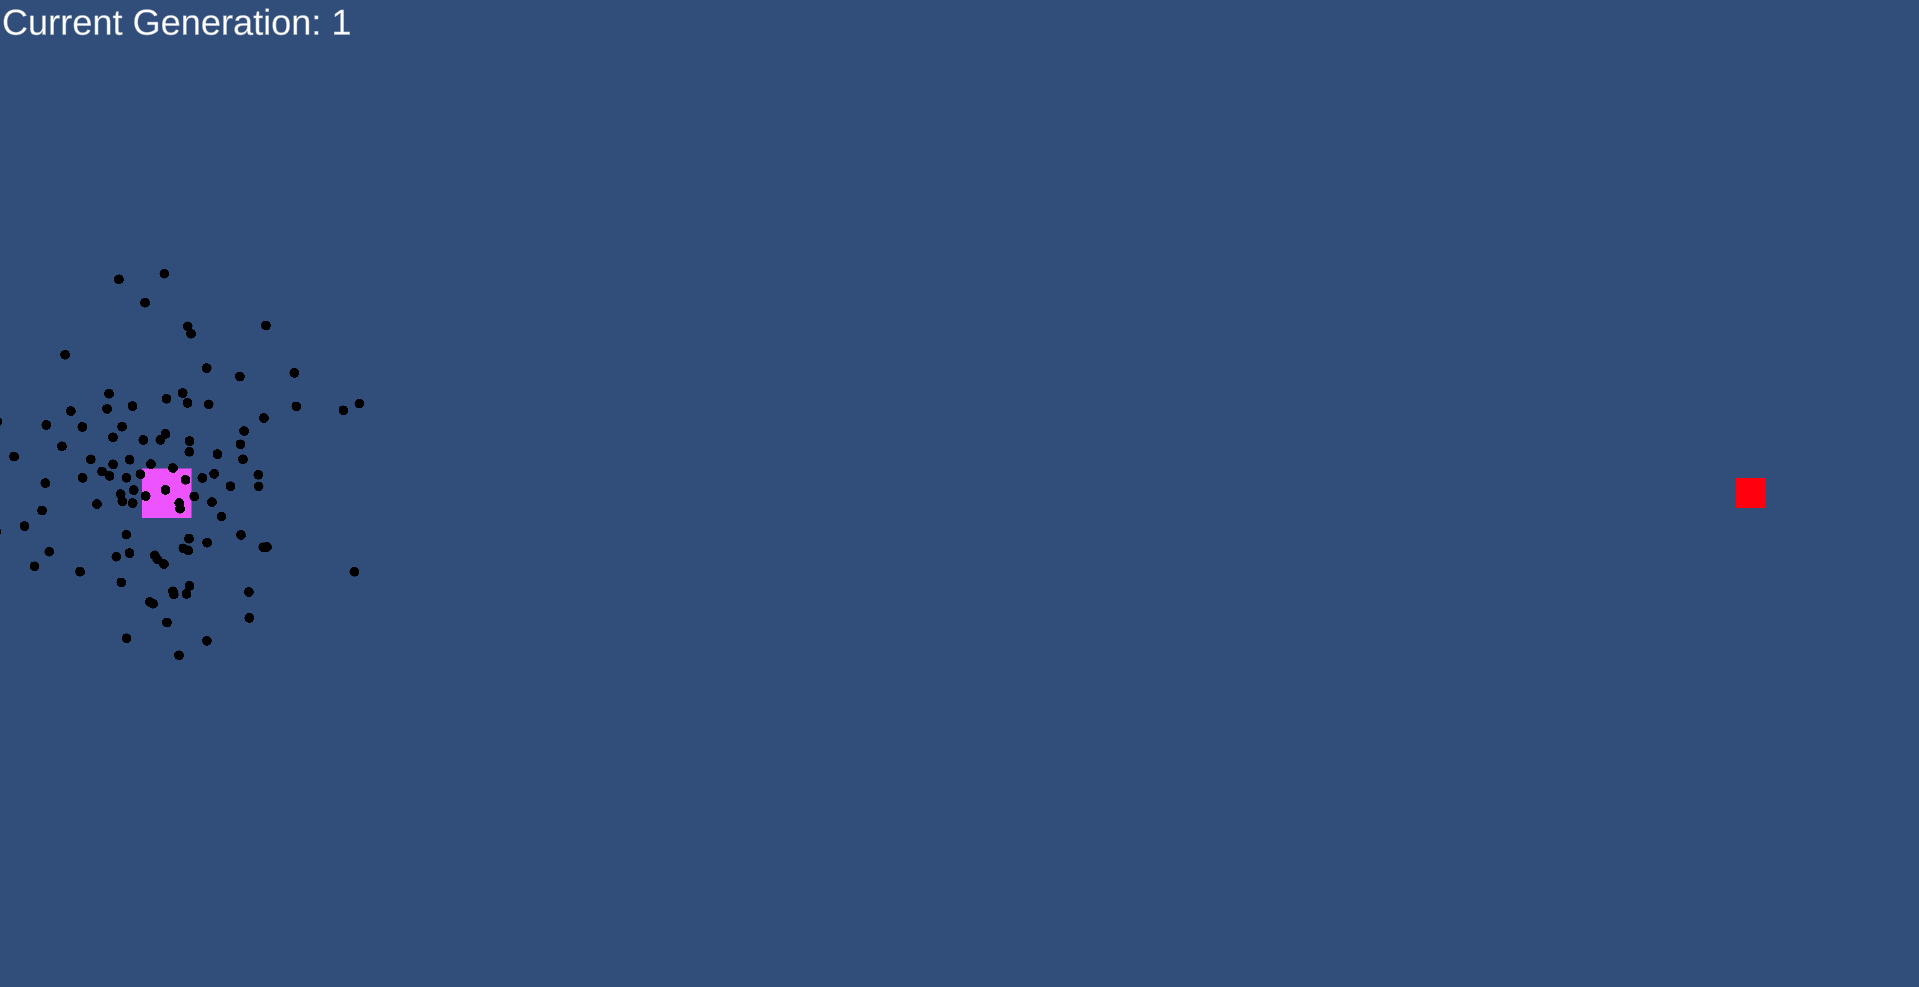
\includegraphics[scale=0.2]{Basic Training - Generation 1}
        \caption {Generation 1}
        \label{fig:Gen1Basic}
    \end{figure}

    \begin{figure}[hbtp]
        \centering
        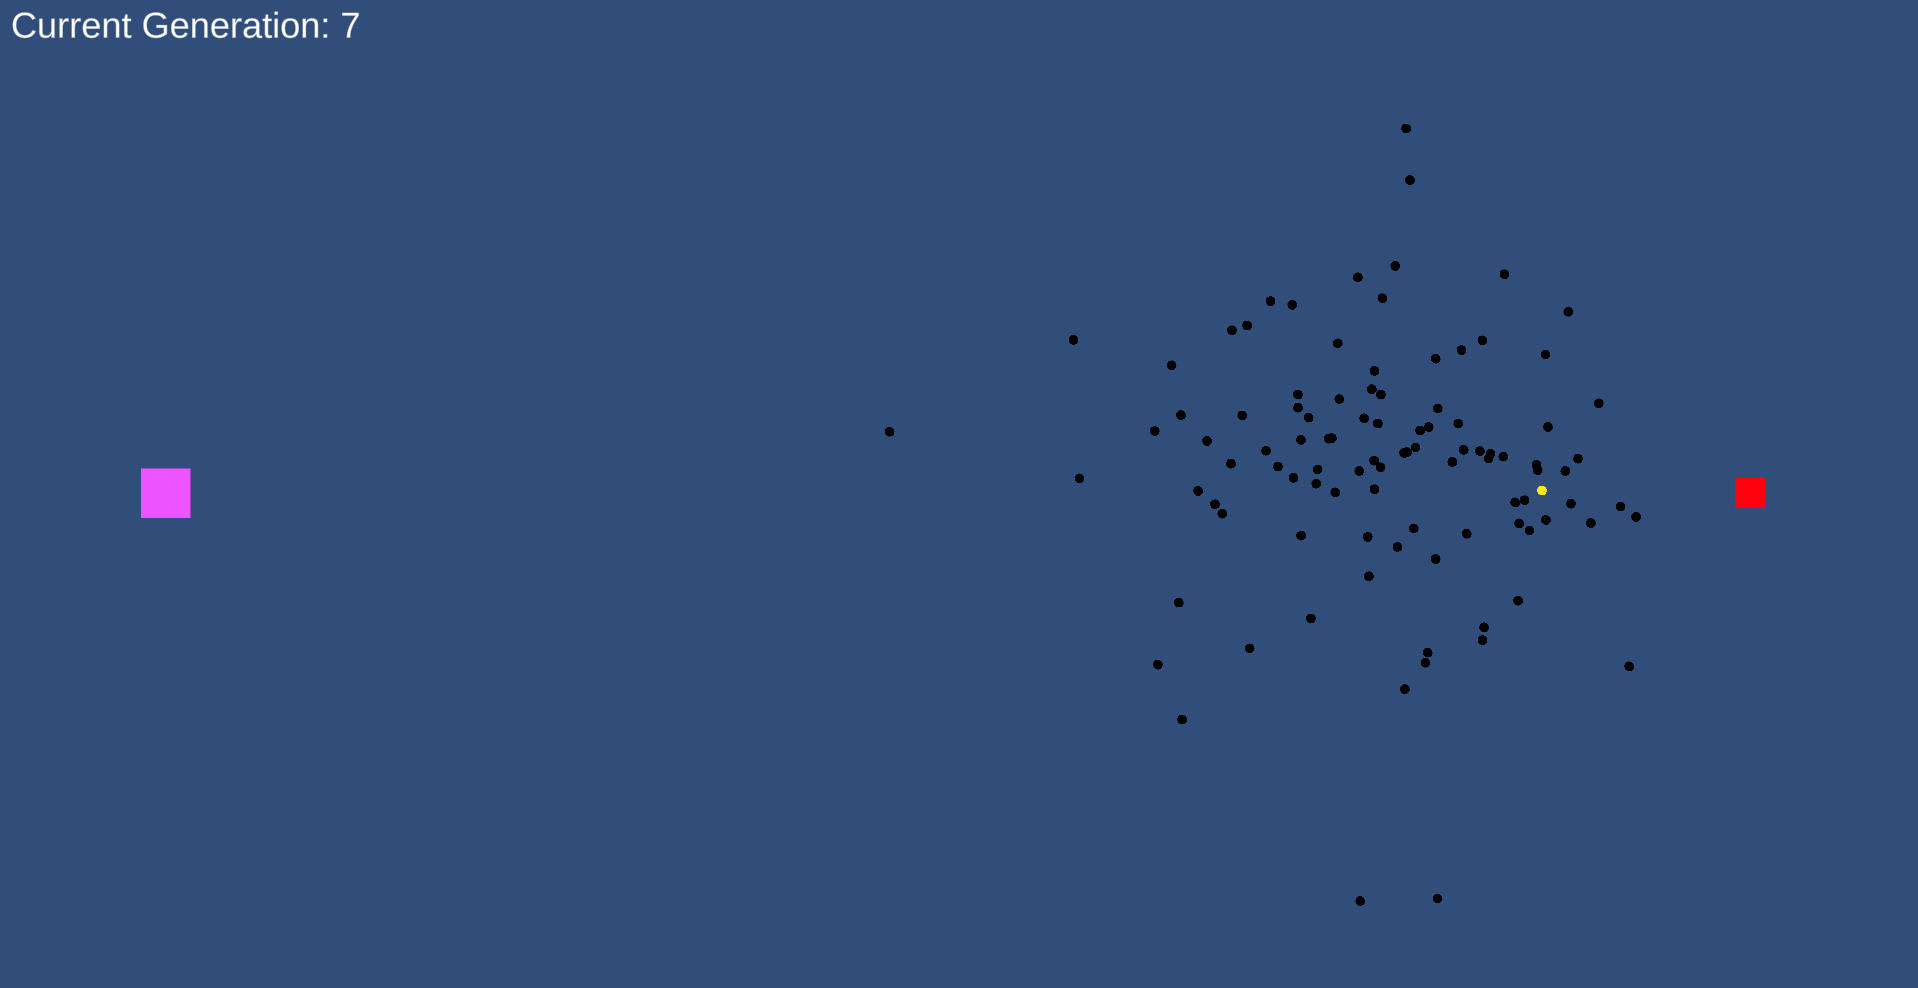
\includegraphics[scale=0.2]{Basic Training - Generation 7}
        \caption {Generation 7}
        \label{fig:Gen7Basic}
    \end{figure}

    \begin{figure}[hbtp]
        \centering
        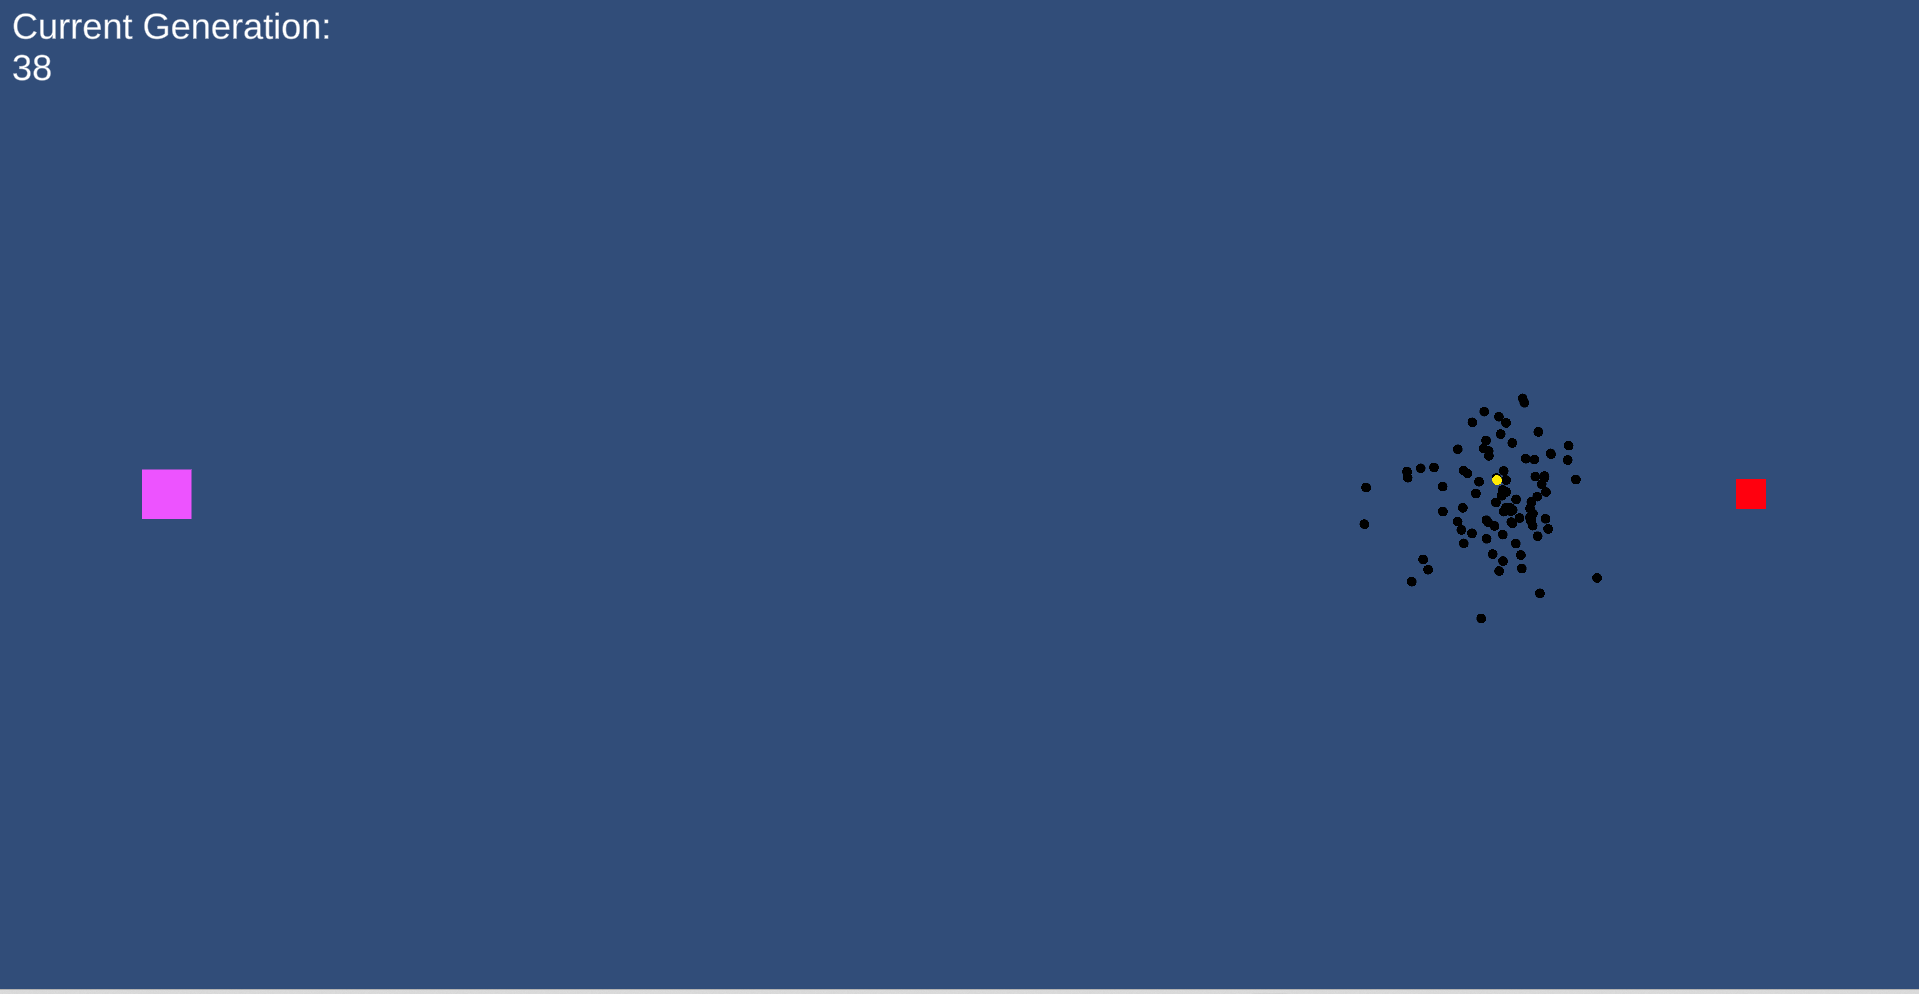
\includegraphics[scale=0.2]{Basic Training - Generation 38}
        \caption {Generation 38}
        \label{fig:Gen38Basic}
    \end{figure}


\end{document}